% vim: set fdm=marker:
\pdfminorversion=4
\documentclass{beamer}

% theme {{{
%\usetheme{Antibes}
\usetheme[compress]{Dresden}
%\usecolortheme{dolphin}
\usecolortheme{rose}
%\usefonttheme{serif}
%}}}

% packages {{{
\usepackage[english]{babel}
\usepackage[utf8]{inputenc}
\usepackage[T1]{fontenc}
\usepackage{caption}
%}}}

% config {{{
%\captionsetup{font=scriptsize,labelfont=scriptsize}
%\renewcommand{\captionfont}{\tiny}
%\renewcommand{\captionlabelfont}{\tiny}
%\setlength{\intextsep}{5.0pt plus 2.0pt minus 2.0pt}
%}}}

% title {{{
\title{Analysis of Image Tranforms for Sketch-based Retrieval}
\subtitle{Diploma Thesis}
\author{Felix Stürmer}
\institute[Fakultät IV - TU Berlin]
{
    Technische Universität Berlin\\
    Fakultät IV - Elektrotechnik und Informatik\\
    Computer Graphics
}
\date{02.11.2012}
\subject{Computer Graphics}
%}}}

\begin{document}
% document {{{

% titlepage {{{
\begin{frame}
  \titlepage
\end{frame}
%}}}

% toc {{{
\begin{frame}{Outline}
  \tableofcontents
  % You might wish to add the option [pausesections]
\end{frame}
%}}}

% introduction and background {{{
\section{Introduction and Background}
\subsection{Motivation}
\begin{frame}{Motivation}
    foo
\end{frame}

\subsection{Challenges of CBIR}
\begin{frame}{Challenges of CBIR}
    \begin{block}{The Semantic Gap}
        \begin{quote}
            ``The semantic gap is the \textbf{lack of coincidence} between the
            information that one can extract from the \textbf{visual data} and
            the \textbf{interpretation} that the same data have for a user in a
            given situation.'' -- Smeulders et al.
        \end{quote}
    \end{block}
    \begin{block}{The Sensory Gap}
        \begin{quote}
            ``The sensory gap is the gap between the \textbf{object in the
            world} and the information in a (computational) description derived
            from a \textbf{recording of that scene}.'' -- Smeulders et al.
        \end{quote}
    \end{block}
\end{frame}

\subsection{Prior Work}
\begin{frame}{Prior Work on Human Recognition}
    \begin{figure}
        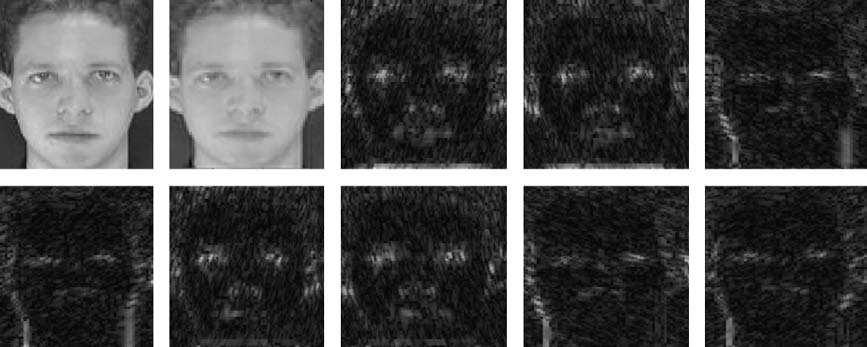
\includegraphics[width=.9\textwidth]{illustrations/related_work/curvelet_faces_mandal09}
        \caption{``Face recognition using curvelet based PCA.'', T. Mandal and Q. M.J Wu, ICPR 2008}
    \end{figure}
\end{frame}

\begin{frame}{Prior Work on Human Recognition}
    \begin{figure}
        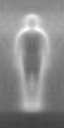
\includegraphics[width=.12\textwidth]{illustrations/related_work/hog_dalal05_1}
        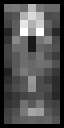
\includegraphics[width=.12\textwidth]{illustrations/related_work/hog_dalal05_2}
        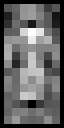
\includegraphics[width=.12\textwidth]{illustrations/related_work/hog_dalal05_3}
        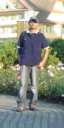
\includegraphics[width=.12\textwidth]{illustrations/related_work/hog_dalal05_4}
        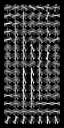
\includegraphics[width=.12\textwidth]{illustrations/related_work/hog_dalal05_5}
        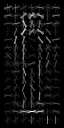
\includegraphics[width=.12\textwidth]{illustrations/related_work/hog_dalal05_6}
        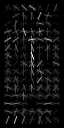
\includegraphics[width=.12\textwidth]{illustrations/related_work/hog_dalal05_7}
        \caption{``Histograms of oriented gradients for human detection'', Dalal and Triggs, CVPR 2005}
    \end{figure}
\end{frame}

\begin{frame}{Prior Work on Visual Codebooks}
    \begin{columns}
        \begin{column}{0.5\textwidth}
            \begin{figure}
                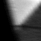
\includegraphics[width=.5cm]{illustrations/related_work/video_google/video_google_dict1_1}
                
\includegraphics[width=.5cm]{illustrations/related_work/video_google/video_google_dict1_2}
                
\includegraphics[width=.5cm]{illustrations/related_work/video_google/video_google_dict1_3}
                
\includegraphics[width=.5cm]{illustrations/related_work/video_google/video_google_dict1_4}
                
\includegraphics[width=.5cm]{illustrations/related_work/video_google/video_google_dict1_5}
                
\includegraphics[width=.5cm]{illustrations/related_work/video_google/video_google_dict1_6}\\
                
\includegraphics[width=.5cm]{illustrations/related_work/video_google/video_google_dict1_7}
                
\includegraphics[width=.5cm]{illustrations/related_work/video_google/video_google_dict1_8}
                
\includegraphics[width=.5cm]{illustrations/related_work/video_google/video_google_dict1_9}
                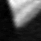
\includegraphics[width=.5cm]{illustrations/related_work/video_google/video_google_dict1_10}
                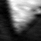
\includegraphics[width=.5cm]{illustrations/related_work/video_google/video_google_dict1_11}
                
\includegraphics[width=.5cm]{illustrations/related_work/video_google/video_google_dict1_12}\\
                
\includegraphics[width=.5cm]{illustrations/related_work/video_google/video_google_dict1_13}
                
\includegraphics[width=.5cm]{illustrations/related_work/video_google/video_google_dict1_14}
                
\includegraphics[width=.5cm]{illustrations/related_work/video_google/video_google_dict1_15}
                
\includegraphics[width=.5cm]{illustrations/related_work/video_google/video_google_dict1_16}
                
\includegraphics[width=.5cm]{illustrations/related_work/video_google/video_google_dict1_17}
                
\includegraphics[width=.5cm]{illustrations/related_work/video_google/video_google_dict1_18}\\
                
\includegraphics[width=.5cm]{illustrations/related_work/video_google/video_google_dict1_19}
                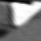
\includegraphics[width=.5cm]{illustrations/related_work/video_google/video_google_dict1_20}
                
\includegraphics[width=.5cm]{illustrations/related_work/video_google/video_google_dict1_21}
                
\includegraphics[width=.5cm]{illustrations/related_work/video_google/video_google_dict1_22}
                
\includegraphics[width=.5cm]{illustrations/related_work/video_google/video_google_dict1_23}
                
\includegraphics[width=.5cm]{illustrations/related_work/video_google/video_google_dict1_24}\\
                
\includegraphics[width=.5cm]{illustrations/related_work/video_google/video_google_dict1_25}
                
\includegraphics[width=.5cm]{illustrations/related_work/video_google/video_google_dict1_26}
                
\includegraphics[width=.5cm]{illustrations/related_work/video_google/video_google_dict1_27}
                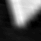
\includegraphics[width=.5cm]{illustrations/related_work/video_google/video_google_dict1_28}
                
\includegraphics[width=.5cm]{illustrations/related_work/video_google/video_google_dict1_29}
                
\includegraphics[width=.5cm]{illustrations/related_work/video_google/video_google_dict1_30}
            \end{figure}
            \begin{figure}
                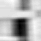
\includegraphics[width=.5cm]{illustrations/related_work/video_google/video_google_dict2_1}
                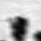
\includegraphics[width=.5cm]{illustrations/related_work/video_google/video_google_dict2_2}
                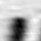
\includegraphics[width=.5cm]{illustrations/related_work/video_google/video_google_dict2_3}
                
\includegraphics[width=.5cm]{illustrations/related_work/video_google/video_google_dict2_4}
                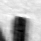
\includegraphics[width=.5cm]{illustrations/related_work/video_google/video_google_dict2_5}
                
\includegraphics[width=.5cm]{illustrations/related_work/video_google/video_google_dict2_6}\\
                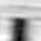
\includegraphics[width=.5cm]{illustrations/related_work/video_google/video_google_dict2_7}
                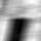
\includegraphics[width=.5cm]{illustrations/related_work/video_google/video_google_dict2_8}
                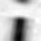
\includegraphics[width=.5cm]{illustrations/related_work/video_google/video_google_dict2_9}
                
\includegraphics[width=.5cm]{illustrations/related_work/video_google/video_google_dict2_10}
                
\includegraphics[width=.5cm]{illustrations/related_work/video_google/video_google_dict2_11}
                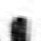
\includegraphics[width=.5cm]{illustrations/related_work/video_google/video_google_dict2_12}\\
                \includegraphics[width=.5cm]{illustrations/related_work/video_google/video_google_dict2_13}
                \includegraphics[width=.5cm]{illustrations/related_work/video_google/video_google_dict2_14}
                \includegraphics[width=.5cm]{illustrations/related_work/video_google/video_google_dict2_15}
                \includegraphics[width=.5cm]{illustrations/related_work/video_google/video_google_dict2_16}
                \includegraphics[width=.5cm]{illustrations/related_work/video_google/video_google_dict2_17}
                \includegraphics[width=.5cm]{illustrations/related_work/video_google/video_google_dict2_18}\\
                \includegraphics[width=.5cm]{illustrations/related_work/video_google/video_google_dict2_19}
                \includegraphics[width=.5cm]{illustrations/related_work/video_google/video_google_dict2_20}
                \includegraphics[width=.5cm]{illustrations/related_work/video_google/video_google_dict2_21}
                \includegraphics[width=.5cm]{illustrations/related_work/video_google/video_google_dict2_22}
                \includegraphics[width=.5cm]{illustrations/related_work/video_google/video_google_dict2_23}
                \includegraphics[width=.5cm]{illustrations/related_work/video_google/video_google_dict2_24}\\
                \includegraphics[width=.5cm]{illustrations/related_work/video_google/video_google_dict2_25}
                \includegraphics[width=.5cm]{illustrations/related_work/video_google/video_google_dict2_26}
                \includegraphics[width=.5cm]{illustrations/related_work/video_google/video_google_dict2_27}
                \includegraphics[width=.5cm]{illustrations/related_work/video_google/video_google_dict2_28}
                \includegraphics[width=.5cm]{illustrations/related_work/video_google/video_google_dict2_29}
                \includegraphics[width=.5cm]{illustrations/related_work/video_google/video_google_dict2_30}
            \end{figure}
        \end{column}
    \end{columns}
\end{frame}

\subsection{Anatomy of a CBIR System}
\begin{frame}{Anatomy of a CBIR System}
    \begin{columns}
        \begin{column}{0.5\textwidth}
            \begin{figure}
                \includegraphics[width=.9\textwidth]{illustrations/cbir_anatomy_query_cropped}
                \caption{Global Descriptors}
                \label{fig:anatomy_global}
            \end{figure}
        \end{column}
        \begin{column}{0.5\textwidth}
            \begin{figure}
                \includegraphics[width=.9\textwidth]{illustrations/cbir_anatomy_query_local_cropped}
                \caption{Local Descriptors}
                \label{fig:anatomy_local}
            \end{figure}
        \end{column}
    \end{columns}
\end{frame}
% }}}

% solution {{{
\section{Proposed Solution}
\subsection{Acquisition}
\begin{frame}{Acquisition}
    \begin{columns}[T]
        \begin{column}{0.5\textwidth}
            \begin{figure}
                \includegraphics[width=\textwidth]{illustrations/input_example_color}
                \caption{Original Image}
            \end{figure}
        \end{column}
        \begin{column}{0.5\textwidth}
            \only<1>{
                \begin{figure}
                    \includegraphics[width=\textwidth]{illustrations/input_example_luma}
                    \caption{Luma Conversion}
                \end{figure}
            }
            \only<2>{
                \begin{figure}
                    \includegraphics[width=\textwidth]{illustrations/input_example_canny}
                    \caption{Canny Operator}
                \end{figure}
            }
            \only<3>{
                \begin{figure}
                    \includegraphics[width=\textwidth]{illustrations/input_example_sobel}
                    \caption{Sobel Operator}
                \end{figure}
            }
            \only<4>{
                \begin{figure}
                    \includegraphics[width=\textwidth]{illustrations/input_example_segment}
                    \caption{gPb-owt-ucm Transform}
                \end{figure}
            }
        \end{column}
    \end{columns}
\end{frame}

\subsection{The Curvelet Transform}
\begin{frame}{The Curvelet Transform}
    foo
\end{frame}

\begin{frame}{The Fast Discrete Curvelet Transform}
    foo
\end{frame}

\subsection{Feature Extraction}
\begin{frame}{Global Feature Extraction}
    foo
\end{frame}

\begin{frame}{Local Feature Extraction}
    foo
\end{frame}

\subsection{Ranking}
\begin{frame}{Ranking}
    foo
\end{frame}
%}}}

% results {{{
\section{Results}
\subsection{Benchmarking}
\begin{frame}{Benchmarking Method}
    foo
\end{frame}

\subsection{Cross-Domain Results}
\begin{frame}{Cross-Domain Results}
    foo
\end{frame}

\subsection{Intra-Domain Results}
\begin{frame}{Intra-Domain Results}
    foo
\end{frame}
%}}}

% conclusion {{{
\section{Conclusions}
\begin{frame}{Conclusions}
    foo
\end{frame}
%}}}

%}}}
\end{document}
